%%%%%%%%%%%%%%%%%%%%%%%%%%%%%%%%%%%%%%%%%%%%%%%%%%%%%%%%%%%%%%%%%%%%%%%%%%%%%%%%
%2345678901234567890123456789012345678901234567890123456789012345678901234567890
%        1         2         3         4         5         6         7         8

\documentclass[letterpaper, 12 pt, conference]{ieeeconf}  % Comment this line out
                                                          % if you need a4paper
%\documentclass[a4paper, 10pt, conference]{ieeeconf}      % Use this line for a4
                                                          % paper

\IEEEoverridecommandlockouts                              % This command is only
                                                          % needed if you want to
                                                          % use the \thanks command
\overrideIEEEmargins
% See the \addtolength command later in the file to balance the column lengths
% on the last page of the document

\usepackage[utf8]{inputenc}
\usepackage[T1]{fontenc}
\usepackage{graphicx}


% The following packages can be found on http:\\www.ctan.org
%\usepackage{graphics} % for pdf, bitmapped graphics files
%\usepackage{epsfig} % for postscript graphics files
%\usepackage{mathptmx} % assumes new font selection scheme installed
%\usepackage{mathptmx} % assumes new font selection scheme installed
%\usepackage{amsmath} % assumes amsmath package installed
%\usepackage{amssymb}  % assumes amsmath package installed

\title{\LARGE \bf
CENG 435 DATA COMMUNICATION AND NETWORKING \\ TERM PROJECT-2 GROUP 75
}

%\author{ \parbox{3 in}{\centering Huibert Kwakernaak*
%         \thanks{*Use the $\backslash$thanks command to put information here}\\
%         Faculty of Electrical Engineering, Mathematics and Computer Science\\
%         University of Twente\\
%         7500 AE Enschede, The Netherlands\\
%         {\tt\small h.kwakernaak@autsubmit.com}}
%         \hspace*{ 0.5 in}
%         \parbox{3 in}{ \centering Pradeep Misra**
%         \thanks{**The footnote marks may be inserted manually}\\
%        Department of Electrical Engineering \\
%         Wright State University\\
%         Dayton, OH 45435, USA\\
%         {\tt\small pmisra@cs.wright.edu}}
%}

\author{Orhan ALBAYRAK$^{1}$ and Mustafa GÖNEN$^{2}$% <-this % stops a space
\thanks{*This report was prepared by Orhan and Mustafa}% <-this % stops a space
\thanks{$^{1}$Orhan is with Department of Computer Engineering, METU - ANKARA e2264471
        {\tt\small}}%
\thanks{$^{2}$Mustafa is with the Department of Computer Engineering, METU - ANKARA e2264547
        {\tt\small www.mustafa.gonenn.com}}%
}


\begin{document}



\maketitle
\thispagestyle{empty}
\pagestyle{empty}


%%%%%%%%%%%%%%%%%%%%%%%%%%%%%%%%%%%%%%%%%%%%%%%%%%%%%%%%%%%%%%%%%%%%%%%%%%%%%%%%
\begin{abstract}

This document is a report was prepared for Data Communications and Networking Term Project in 2019. 

\end{abstract}


%%%%%%%%%%%%%%%%%%%%%%%%%%%%%%%%%%%%%%%%%%%%%%%%%%%%%%%%%%%%%%%%%%%%%%%%%%%%%%%%
\section{PROJECT OVERVIEW}

\subsection{ Overview }

In this project our main goal is to design and implement the nodes of a network topology that the components are Source, Router-1, Router-2, Router-3 and Destination. In this part (Part-2), we implement two experiments. In this concept. We implement our (RDT) protocol in the App. Level. 
\vspace{1cm}

The other specifications that we will have followed that; using UDP (User Datagram Protocol) socket programming features based Reliable Data Transfer (RDT) in these implementations. So, we need to translate the data reliable way from source to destination.  Because we know that unlike TCP, UDP does not provide us reliability. For instance, the case of the possibility of link failure we should transmit data another way or the case of the possibility of bit error we should re transmit the data which the error emerges etc. To reach correct data from destination part we have used "md5sum" for checksum and the case of link lost or correctness transmitting process we look at timeout mechanism for handle it. Thanks to pipe-lining and multi-homing file will be transmitted more efficient way.

\subsection{ Experiment 1 }

In first one (Experiment-1) is about that we have used the shortest path that we already found in Part-1 with Dijkstra’s Algorithm. At this stage, out path is used Source, Router-3 and Destination. On this path a large (5 MB) should transmitted on followed path (Just one router). In this scenario, the role of the router is that just transferring data with UDP Based Protocols receiving from source and sending to destination  \\ \\
Path: Source --> Router-3 --> Destination \\

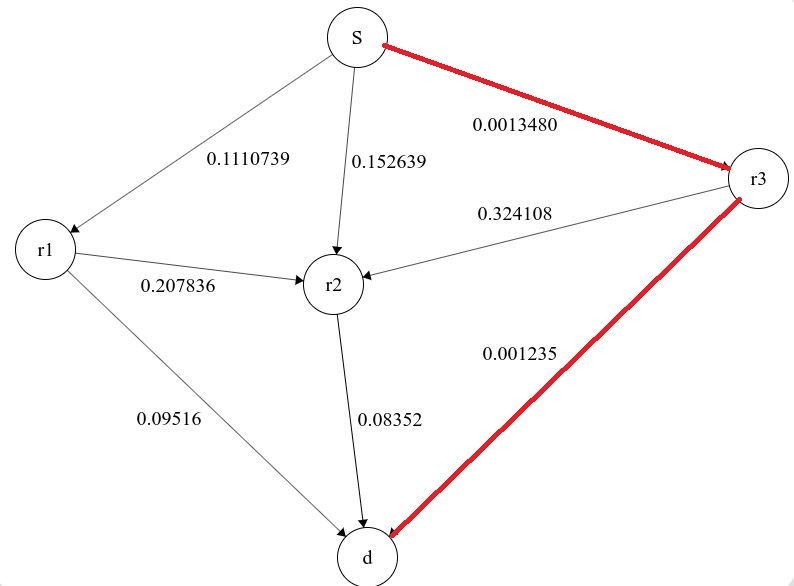
\includegraphics[width=8.5cm, height=7cm]{shortest-path.jpeg}

\begin{center}
Figure-1
\end{center}
\\
\subsection{ Experiment 2 }

And Experiment-2 we add the source implementation to do multi-homing. That is provide our network more reliable; since possibility of link failure source should transmit the data over another path(If Router-1 could be down then source should send data over Router-2 and if Router-2 could be down then source should send data over Router-2 to destination). At this stage, our path is should be Source, Router-1 or Router-2 and Destination. This stage was harder to handle than the first experiment. \\ \\
Path: Source -->   Router-1   --> Destination \\
Path: Source -->   Router-2   --> Destination \\

In both experiment the main goal was similar. Basically, after reading the file at source we divide them as packets and adding some information in them as bytes then send them to routers. After routers receive them their duty is just forwarding the data to destination and forwarding the ACKs to source. 
\vspace{1cm}

We control the reliability of the channel with checksum and timeout mechanisms. After each packet is send from source timeout is set then wait to its ACK packet. If the ACK is not received the source side in the expected time (that we set in the timeout) or if the packet checksums are not matched, then we understood and handle the error by sending the ACK number of the penultimate packet. (In Design Approach and Implementation part we handle these topics more detailed).
\vspace{1cm}

At the beginning of the working we shared the workload. But this working still is not seemed logically. Because in this way we could not coordinate and suffered while communicating. Then we decide to work together, and we met in department. We shared the all parts of assignment workload throughout the project. 
\vspace{1cm}

Firstly, we decided the design and architecture then we have done configurations and thought how we should do the experiments and how can we find solutions of the problems that we encountered while implementing, understanding and fixing. When we stuck, we consulted to forums sites and our lecture slides. In this perspective we decided to implement like go back N protocol. The implementations of node’s scripts are developed by both group member. After implementations we completed experiment, README file and finally report writing.
More detailed explanations are handled in follow.
\vspace{1cm}

\section{ Design Approach }
Our problem was transferring a file of 5 MB from source to destination over router in correct order and reliable way by using UDP. Because we have to use UDP to provide the reliability by implementing some mechanisms on source and destination nodes. 
\vspace{1cm}

For sending file source to destination we have two way. One is we use Experiment-1 and other one is Experiment-2. Let’s look these experiments close window.
\vspace{1cm}

\subsection{Experiment 1}
In Experiment-1 we send a file (5 MB) from source node to destination node over router-3. In the source node firstly, this file is read from input.txt file which we downloaded from assignment page. Then we divide this large file to chunks because we should transmit this file packet-based mechanism and because of we could not transmit bigger than 1000 byte. After divided file to checking the correctness of chunks content we add this file a checksum information. To get that we created a hash object that is obtained from md5sum. Then this information is packed for adding to data in byte format. Then for tracking the packets we add them a sequence number which are packed same way as checksum hashes.
\vspace{1cm}

The final packet is consisting of packet’s sequence number, hash of the data checksum, and data itself (seq. number + checksum + data). After creating this package source sends it to Router-3. Then source starts to be waiting an answer from router-3 to understand to whether data is received from destination or not. With this control if the same ack number is returned to source and the unpacked hash is matched at the destination part then we can understand that packet is send to destination successfully (There is no bit error or packet loss). 
\vspace{1cm}

Hovewer what happens if the penultimate sequence number is received to source. Beside of this we could not wait the acknowledge message for a long time. So, we set the timeout (timeout mechanism is used here) and the case of the ack number is could not received from source in this interval, we will send the same packet again. This feature provides us reliable data transfer (RDT). And these steps are followed until the all file is transferred to destination. 

In router side issues are solved straightforward way. It is waiting data from source. At the time of receiving data it just forward data to destination. Because it in not responsible for examining the content of the packet. Its duty just transferring the data what it is received. So, Router-3 take data from source and transmit it to destination and take the ack number of the packet which it has forwarded from destination and send it to source.
\vspace{1cm}

In destination side it listens router. When a packet received it unpacks the coming packet to hash information, sequence number and data itself. After unpacking process, it compares the coming hash information with hash information of the data which it has received. After comparison destination create an acknowledgment number to tell source that I have received data correctly and no corruption. After these processes if there is bit error it sends last packet’s sequence number which it received correctly. Beside of this if there is no coming packed in dedicated time interval destination node assumes that there is packet loss and it want to next packet from source over router-3 in same manner.
\vspace{1cm}

After these processes we send the input.txt file from source and received it in destination node in a successful way and write it to output file. (We compare them in terminal with diff command)
	
	\subsection{Experiment 2}
	
In Experiment-2 our goal is same in Experiment-1. We should send a file (5 MB) from source node to destination node over router-1 or router-2. So, in this experiment our components are source, router-1, router-2 and destination. The sending process are handled with the two links (router-1 and router-2) at the same time. While sending packets destination we chose the routers if the sequence number is odd then packet is transmitted over router-1 and if the sequence number is even then packet is transmitted over router-2. This called as Multi-homing. It provides us more reliable and more efficient processes. Because if one link will down then we will send the data other path so it provides reliability. We assume that in this experiment data will transferred to destination faster than first experiment because of the two links usage effect the transmission exponential.
\vspace{1cm}

Firstly, in source node the input.txt file is read. Then we divide it like in experiment-1. When the sending them to routers we chose the link regard as packet’s sequence numbers as I said. After sending process we check the links whether they are still alive or not. The case of the link-down or link failure we will send the remaining packets to destination over the link which is still alive. Beside of these operation source waits the ACK message from destination over router-1 and router-2 to understand whether the packets are transmitted successfully or not. The case of the failure it sends same packets again and again. 
\vspace{1cm}

In router side we implement the same scripts in both router and both experiments. Since, as I said their main purpose is forwarding the file which they received. They have two sockets when one is waiting data from the source and response it with ACK message and the other one is sending the data that it received to destination and receiving the coming ACK number. They have not any complicated role they don’t change anything about data.
\vspace{1cm}

In the destination node, we are listening data from two routers: router1 and router2. It checks the routers usability with if block is router-1 still alive and is router-2 still alive. When a link is down destination just continue to listen other link and receive all packets. When a packet is received with the expected ack number from the router to this node, it does a check process for bit error , the same ack no is sent back to router-1 or router-2 that means that it destination node is waiting the same packet again. If the timeout occurs, one link is down so we should not listen it anymore. In addition that because of the we have not any buffer implementation in here we simply discard the packet. So we write only the packets that is received on output file .
\vspace{1cm}	

\section{IMPLEMENTATION PART}

\subsection{Introduction}

We have used Python3 in our Project as programming Language because  Python has lots of library which helps us about Socket Programming and Threading. And also it is more useful  for development.  We preferred different scripts for each node and for each experiments. In this way we have done more possible  to understand our variables, functions,  inputs outputs etc.
\vspace{1cm}

\subsection{Platform}
About GENI Platform, we did not do anything new to us.  After uploading our topology on GENI Platform, we could able to access all nodes,links and interfaces easily. Although we did not design experiments (1 and 2) differently we will work for on them separately.
\vspace{1cm}

\subsection{Implementation Process}
We know these concepts(client and server applications in Python Socket Programming, creating socket function, closing socket function, sending a random message from client to server and receiving response from server) from Phase 1 it was easier for us to overview these concepts . After passing this concepts, we have designed a client/server application between source node and router-1. We developed two script 'source.py' for source node 'r3.py' for router-3 for this application. In these scripts, we have mainly tried sending and receiving a large size data 5MB (input.txt) between source and router-3. 
\vspace{1cm}

For experiment 1, we have developed 3 different scripts (source.py router-3.py and destination.py).
\vspace{1cm}

In source.py script, we have created a UDP socket for transferring our packets to router-3. Then, we defined our port number and IP addresses for server and client. After this defining, we opened the file named input.txt, size 5MB with read-only mode. Then, we started to reading file step by step. In this stage, we determined our data packet size is 900 byte. We are sending data with encapsulation method using "struct.pack" function in struct library. In this packing method, we packed three elements "Sequence Number of packet + hashing of packet + content of data. Content of data is a 900 byte size packet from "input.txt". Sequence Number is number for identifier of a packet and Hashing of packet is checksum of a packet that we create using "hashlib" function importing hashlib library. After creation of these information we have encapsulated, we have sent our data from "source" to "router-1" with address information using "sendto" function.
\vspace{1cm}

In router.py, router has no important role in this design. It just only, receive and send data like a bridge between source and destination. To be able to do it, it needs client and server ip address for source and destination and two different port number for each link.
\vspace{1cm}

In destination.py, unpacking that encapsulated packet with (hash,seq number and data content) information has very important role not to be lost and info. We opened this packet content with using "unpack" function. According to our packing methods,\\
ack-number --> struct.unpack("d", data[:8])[0]\\
unpacked-hash = struct.unpack("32s", data[8:40])[0].decode("utf-8")\\
data --> data[40:]\\
After we obtained these information of data, we have checked whether is same hashing of packet before and after. If they are completely same, we have understood that that packet is transmitted without any loss. Then, we checked seq and ack number.
\vspace{1cm}

In experiment 2, we did not use different logic from experiment 1. We have same input.txt file (5MB). However, we have used two different path:\\\\
Path: Source -->   Router-1   --> Destination \\
Path: Source -->   Router-2   --> Destination \\
\vspace{1cm}

We have designed "timeout" property using functions sock.settimeout(time) in the code. We used Router-1 the packets which has even sequence number while have used Router-2 the packets which has odd sequence numbers. We designed this stage to avoid link failure as much as possible.

\subsection{ Paths in Experiment 1 and Experiment 2 }
\begin{center}
Experiment 1
\end{center}

\begin{center}
 \begin{tabular}{||c c||} 
 \hline
 Destination & Send to  \\ [0.25ex] 
 \hline\hline
 S & R3  \\ 
 \hline
 R3 & D  \\

 
 \hline
\end{tabular}
\end{center}

\vspace{6cm}
\begin{center}
Experiment 2 (a)
\end{center}

\begin{center}
 \begin{tabular}{||c c||} 
 \hline
 Destination & Send to  \\ [0.25ex] 
 \hline\hline
 S & R1  \\ 
 \hline
 R1 & D  \\
 
 \hline
\end{tabular}
\end{center}
\vspace{1cm}
\begin{center}
Experiment 2 (b)
\end{center}

\begin{center}
 \begin{tabular}{||c c||} 
 \hline
 Destination & Send to  \\ [0.25ex] 
 \hline\hline
 S & R2  \\ 
 \hline
 R2 & D  \\
 
 \hline
\end{tabular}
\end{center}


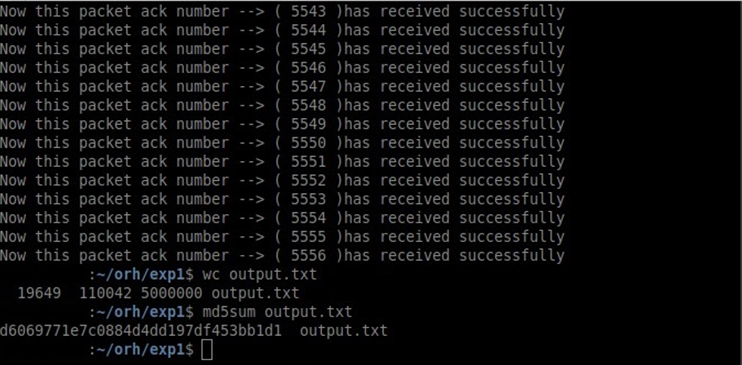
\includegraphics[width=8.5cm, height=7cm]{Experiment 1-dest.png}

\begin{center}
Experiment 1 Destination
\end{center}

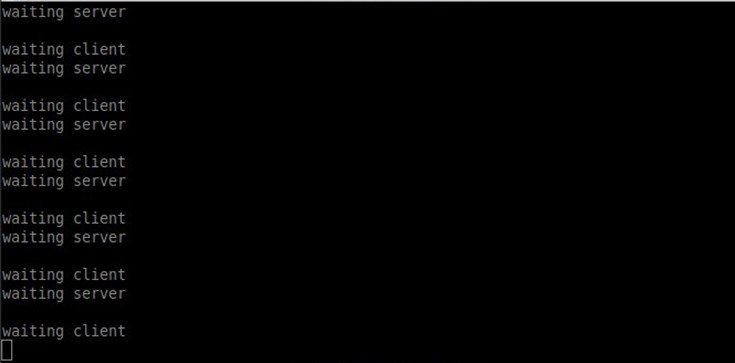
\includegraphics[width=8.5cm, height=7cm]{Experiment 1-r3.png}

\begin{center}
Experiment 1 Router-3
\end{center}


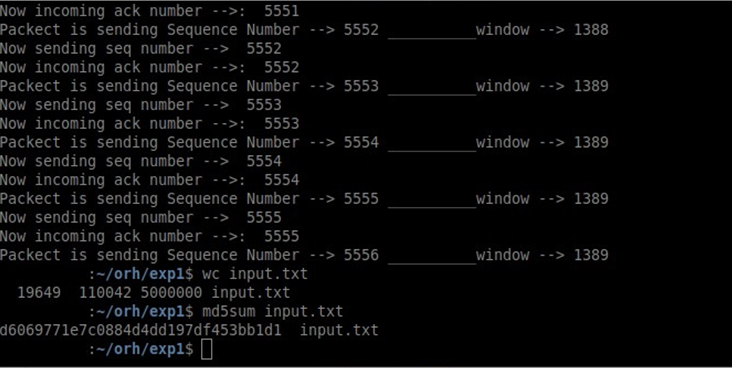
\includegraphics[width=8.5cm, height=7cm]{Experiment 1-source.png}

\begin{center}
Experiment 1 Source
\end{center}


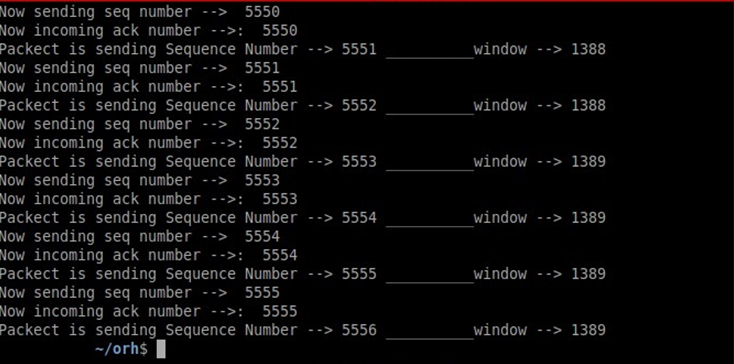
\includegraphics[width=8.5cm, height=7cm]{Experiment 2-a-source.png}

\begin{center}
Experiment 2-a Non-stop Source
\end{center}


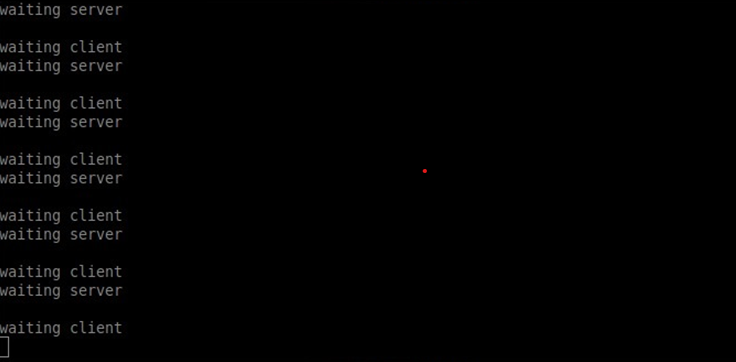
\includegraphics[width=8.5cm, height=7cm]{Experiment 2-a-r1.png}

\begin{center}
Experiment 2-a Non-stop Router-1
\end{center}


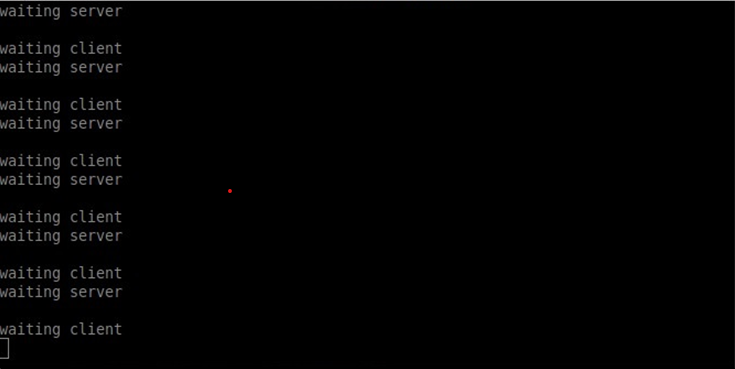
\includegraphics[width=8.5cm, height=7cm]{Experiment 2-a-r2.png}

\begin{center}
Experiment 2-a Non-stop Router-2
\end{center}

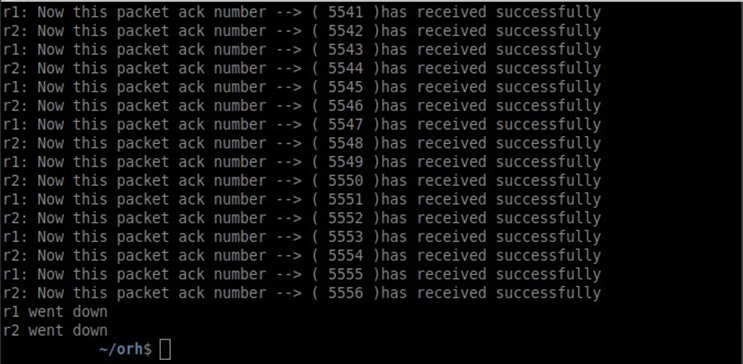
\includegraphics[width=8.5cm, height=7cm]{Experiment 2-a-dest.png}

\begin{center}
Experiment 2-a Non-stop Destination
\end{center}



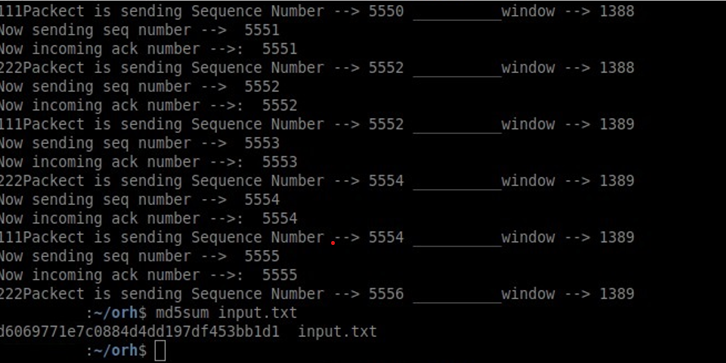
\includegraphics[width=8.5cm, height=7cm]{Experiment 2-b-sourcepng.png}

\begin{center}
Experiment 2-b Link Down Source
\end{center}


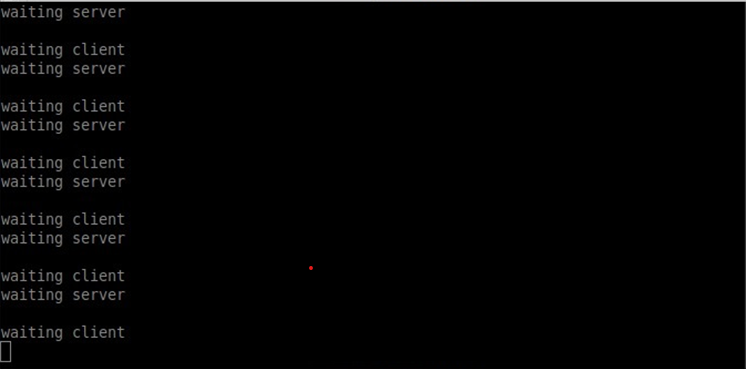
\includegraphics[width=8.5cm, height=7cm]{Experiment 2-b-r1.png}

\begin{center}
Experiment 2-b Link Down Router-1
\end{center}


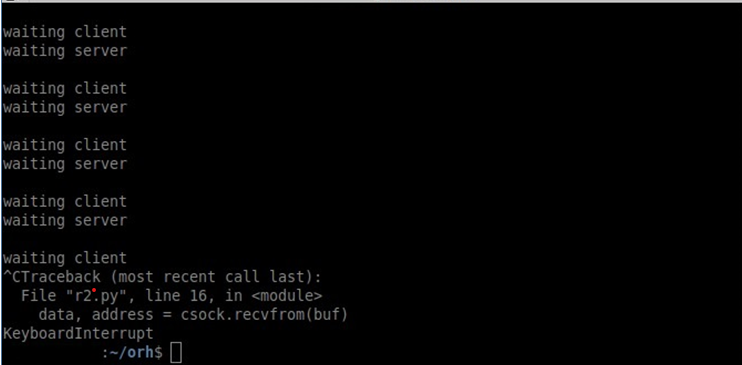
\includegraphics[width=8.5cm, height=7cm]{Experiment 2-b-r2.png}

\begin{center}
Experiment 2-b Link Down Router-2
\end{center}

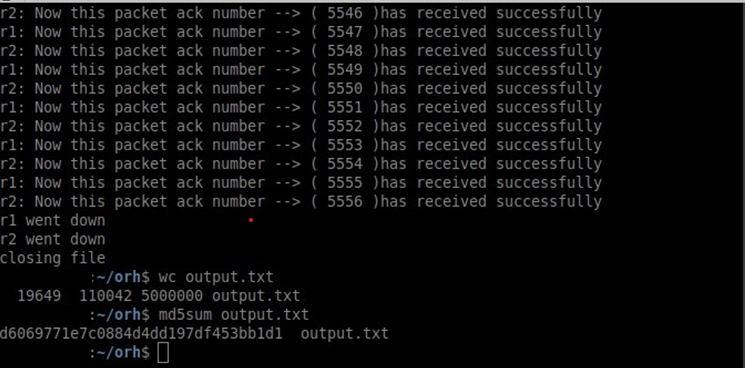
\includegraphics[width=8.5cm, height=7cm]{Experiment 2-b-dest.png}

\begin{center}
Experiment 2-b Link Down Destination
\end{center}



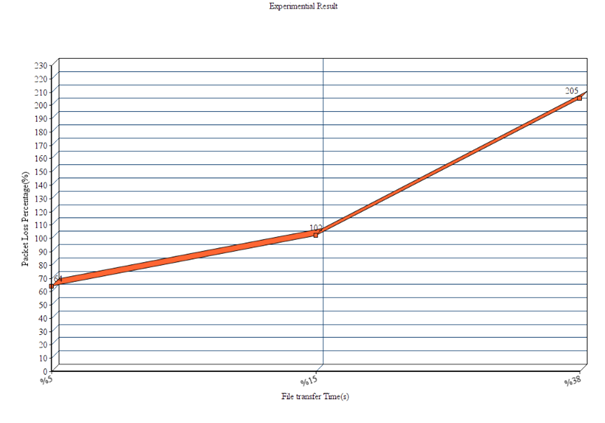
\includegraphics[width=8.5cm, height=7cm]{Graph.png}

\begin{center}
Packet Lost vs. File Transfer Time Graph
\end{center}

\vspace{5cm}

We can see obviously when the increasing packet loss the file transfer time is increasing significantly. However, we can transfer all the file even the packet loss increases. Now if we are looking close window to our two experiment while packet loss increasing multi homed data transformation is more efficient and successful way. We know that in first experiment we are using shortest path. Despite this situation, when the 38 packet loss percentage file transferring experiment take more time in experiment-1 than the experiment-2. So how it can be happening? For experiment two our source code connected to router-1 and router-2. So, packets are transferring in two links to destination. When one of the links down and the transfer will continue from the other link which is still alive. 








\end{document}



